\section{Method}
\label{sec:method}

Fig.~\ref{fig:pipeline} shows what goes in and what comes out: reasoning turns the clip into an ontology and candidate variations, guidance turns one variation into a prompt and four control maps, and generation renders it. The only manual decision is which variation to render. A clip is a frame sequence $V=\{I_t\}_{t=1}^{T}$ with $T=60$ at 4~fps and $854\times480$ pixels. The reasoning model $R$ maps the first frame to an ontology $\mathcal{O}=R(I_1)$: a task record, objects $\{o_k\}$ with normalized boxes $b_k\in[0,1000]^4$, and for each object candidate variations $\mathcal{U}_k$ such as ``solid blue matte.'' The prompt writer $L$ maps $(\mathcal{O},u)$ to a prompt $p$ for a chosen $u\in\mathcal{U}_k$; the segmenter $S$ maps a box and the clip to a tracked binary mask $S(b_k,V)\in\{0,1\}^{T\times H\times W}$; the generator $G$ maps $(V,p,\{c_j\},w)$ to a variant $V'$, where $c_j$ are control videos and $w$ their weights.

\begin{figure}[t]
\centering
\begin{tikzpicture}[
  font=\scriptsize,
  inbox/.style={draw, rounded corners=2pt, fill=black!4, text width=42mm, inner sep=3pt, align=left, minimum height=7mm},
  core/.style={draw, rounded corners=2pt, fill=green!12, text width=20mm, align=center, inner sep=3pt},
  outbox/.style={draw, rounded corners=2pt, fill=black!4, text width=33mm, align=center, inner sep=3pt},
  arr/.style={-{Latex[length=1.6mm]}, thick}
]
\node[inbox] (clip) {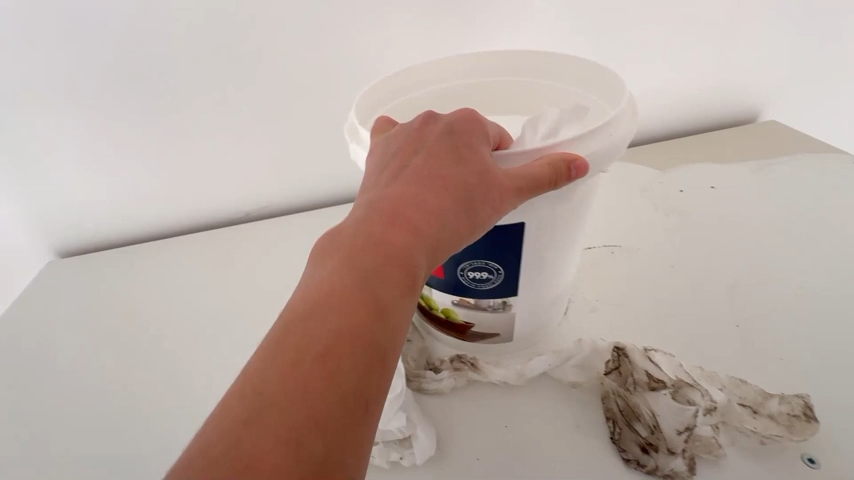
\includegraphics[height=6mm]{s03_original.png}\hspace{2pt}\begin{minipage}[b]{30mm}Original clip $V$\\60 frames, 4 fps\end{minipage}};
\node[inbox, below=1.5mm of clip] (prompt) {Ontology $\mathcal{O}$ + text prompt $p$};
\node[inbox, below=1.5mm of prompt] (maps) {Four guidance maps $c_j$: edges, depth, color, seg,\\with weights $w$ that balance them};
\node[inbox, below=1.5mm of maps] (mask) {Subtraction mask $M$: where the model should paint};
\node[core, right=7mm of $(prompt.east)!0.5!(maps.east)$] (tr) {\textbf{Cosmos Transfer 2.5}\\video-to-video generation};
\node[outbox, right=7mm of tr] (out) {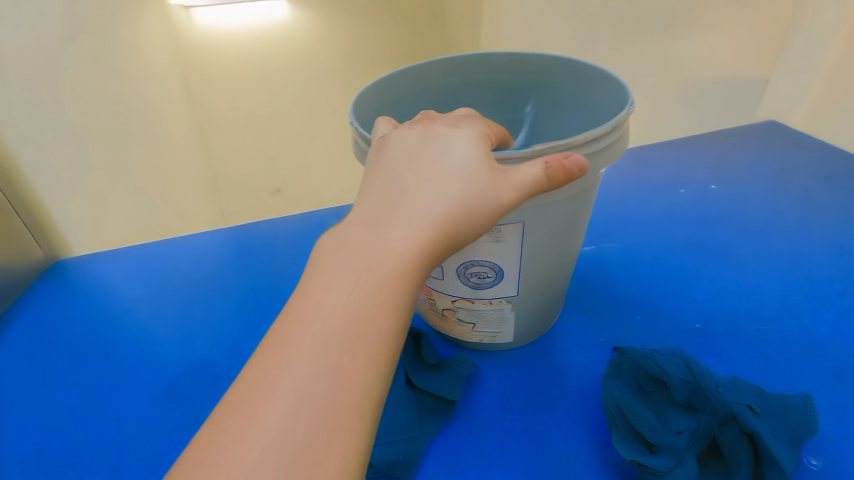
\includegraphics[width=30mm]{s04_created.png}\\Synthetic clip $V'$: same task, same actions, new appearance};
\coordinate (bus) at ($(clip.east)+(3.5mm,0)$);
\foreach \n in {clip,prompt,maps,mask} {\draw[thick] (\n.east) -- (\n.east -| bus);}
\draw[thick] (clip.east -| bus) -- (mask.east -| bus);
\draw[arr] (tr.west -| bus) -- (tr.west);
\draw[arr] (tr) -- (out);
\end{tikzpicture}
\caption{Pipeline. Every input to the renderer is produced by an earlier stage: the ontology and prompt by the reasoning model and the language model, the guidance maps by the preprocessors shipped with Transfer, and the mask by SAM2 from the ontology's boxes.}
\label{fig:pipeline}
\end{figure}

\subsection{Reasoning with Structured Ontologies}
\label{sec:reason}
Domain randomization swaps colors and textures at random and hopes the policy learns to ignore them. Our premise is that the model should first understand the scene, so that a bucket in a cleaning clip is a cleaning bucket and not a bucket on a shelf. We prompt the reasoning tower of Cosmos 3 Nano~\cite{cosmos3} (16B parameters, 8B in the tower) with the first frame and a fixed instruction asking for up to ten task-relevant objects with boxes and an exhaustive list of variations along seven dimensions per object (color, material, size, state, condition, interaction, brand). The answer is JSON in a fixed schema (Fig.~\ref{fig:ontology}). \texttt{role\_in\_task} conditions the variations on what the object is for; \texttt{robustness\_gaps} lists failure modes such as the bucket tipping over, which are changes of action and go to a different renderer (Sec.~\ref{sec:generation}). The raw count exceeds 100 per clip; 72 on average survive the filter below.

\begin{figure}[t]
\centering
\begin{minipage}[c]{0.31\linewidth}
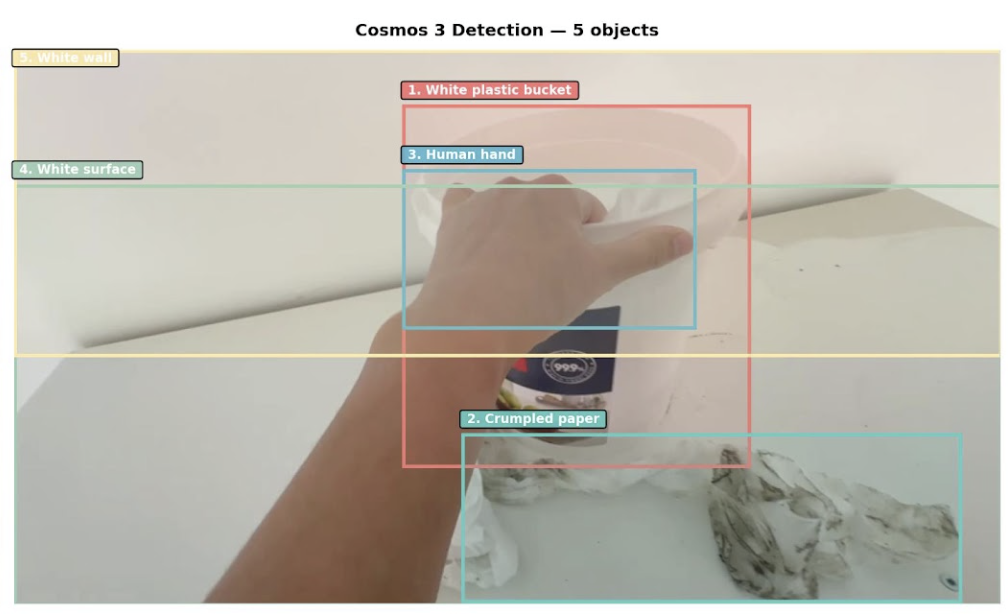
\includegraphics[width=\linewidth]{s08_detection.png}
\end{minipage}\hfill
\begin{minipage}[c]{0.67\linewidth}
\begin{lstlisting}
"task": { "name": "Disposing of crumpled paper into a bucket",
  "action_primitive": "Holding a bucket and positioning it" },
"key_objects": [{ "name": "White plastic bucket",
  "role_in_task": "Container for disposing of waste",
  "robustness_gaps": {
    "what_robot_must_handle": ["Different bucket sizes and shapes",
      "Labels with varying colors and designs", "Wet or slippery buckets"],
    "common_failure_modes": ["Bucket slips from hand",
      "Bucket tips over", "Bucket cannot be opened"] } }]
\end{lstlisting}
\end{minipage}
\caption{Reasoning output for the running example: five task-relevant objects with boxes, and an excerpt of the bucket's record. The task name is wrong (the clip shows wiping) and ``bucket cannot be opened'' is implausible for an open bucket; the filter stage exists to catch such entries.}
\label{fig:ontology}
\end{figure}

\subsection{From Ontology to Generation-Ready Prompts}
\label{sec:prompts}
GPT-4o mini~\cite{gpt4omini} keeps the variations that pass six plausibility checks (material against the task's contact forces, object size against the scene, material against the room type, physical possibility, lighting against time of day, and whether the object belongs in such a scene) and writes the Transfer prompt, which for the running example begins ``The video captures a person cleaning a solid blue countertop in a well-lit indoor kitchen\ldots\ The bucket and paper towels retain their original appearance.'' Three rules found by trial are encoded in the instruction: repeat the target attribute two or three times and name the material, not just the color; name every object that must stay unchanged; and describe the result as a scene rather than an edit, because Transfer was trained on captions of the output, not on instructions. Sec.~\ref{sec:leakage} measures how well the second rule holds.

\subsection{Guiding the Renderer}
\label{sec:guidance}
Transfer receives four control videos, each protecting a different part of the source (Fig.~\ref{fig:maps}, top). Canny edges $c_{\mathrm{edge}}$~\cite{canny1986} keep the shapes, so the bucket stays a bucket; monocular depth $c_{\mathrm{depth}}$~\cite{depthanything} keeps the layout; a heavily blurred copy of the source $c_{\mathrm{vis}}$ keeps the palette and lighting; a segmentation video $c_{\mathrm{seg}}$ says where to paint. The first three come from the preprocessors shipped with Transfer. The fourth needs one extra step, because the surface to recolor overlaps the bucket, towels and hand that must not change. SAM2~\cite{sam2} returns a tracked mask for the surface box $b_{\mathrm{surf}}$, which includes whatever lies on the counter, and one for each object box $b_k$; the final mask is
\begin{equation}
    M_t = S(b_{\mathrm{surf}},V)_t \;\setminus\; \bigcup_{k} S(b_k,V)_t ,
    \label{eq:mask}
\end{equation}
computed per frame on SAM2's propagated masks, so $M$ is temporally consistent without a separate tracker (Fig.~\ref{fig:maps}, bottom). $M$ enters Transfer as $c_{\mathrm{seg}}$. It is a control signal, not painter's tape: the model follows it to the degree set by the seg weight, and nothing forbids change outside $M$. The weights $w$ are the one set of hyperparameters we tuned, by moving each until a failure appeared and backing off (Table~\ref{tab:weights}). Edges matter most and are pinned on both sides; color guidance must be nearly off, because it conditions on the source colors and opposes any recolor.

\begin{figure}[t]
\centering
\begin{subfigure}{0.24\linewidth}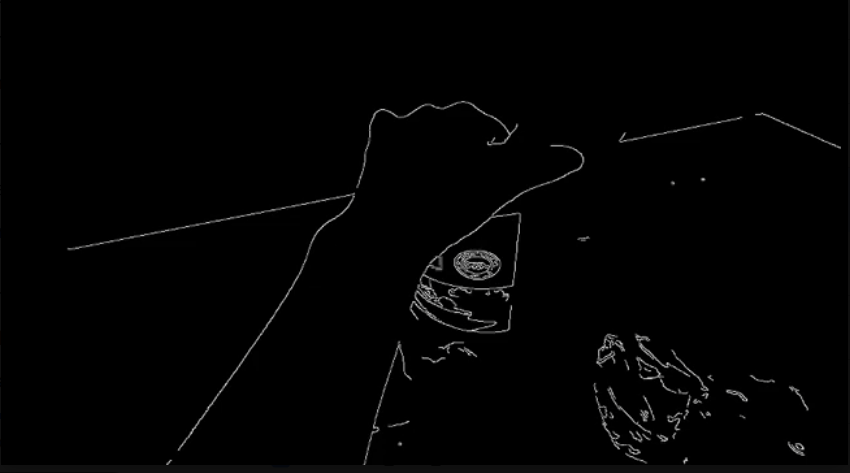
\includegraphics[width=\linewidth]{s10_edges.png}\caption{edges}\end{subfigure}\hfill
\begin{subfigure}{0.24\linewidth}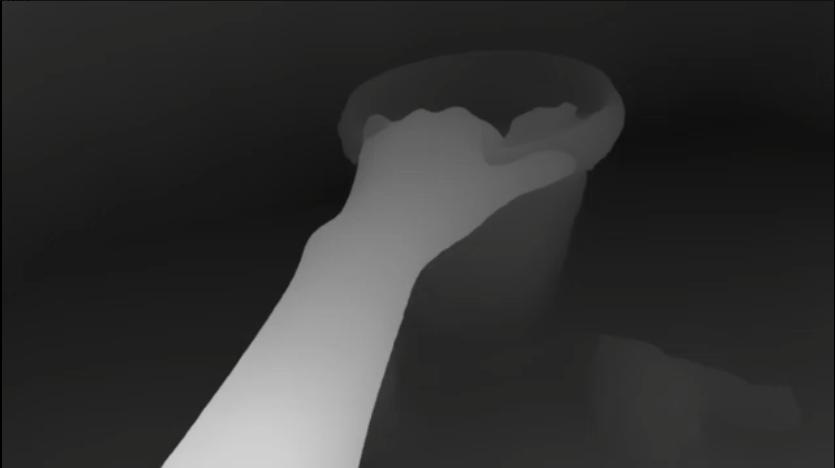
\includegraphics[width=\linewidth]{s10_depth.png}\caption{depth}\end{subfigure}\hfill
\begin{subfigure}{0.24\linewidth}
\includegraphics[width=\linewidth]{s10_color.png}\caption{color (vis)}\end{subfigure}\hfill
\begin{subfigure}{0.24\linewidth}
\includegraphics[width=\linewidth]{s10_mask.png}\caption{mask (seg)}\end{subfigure}\\[1.5mm]
\begin{subfigure}{\linewidth}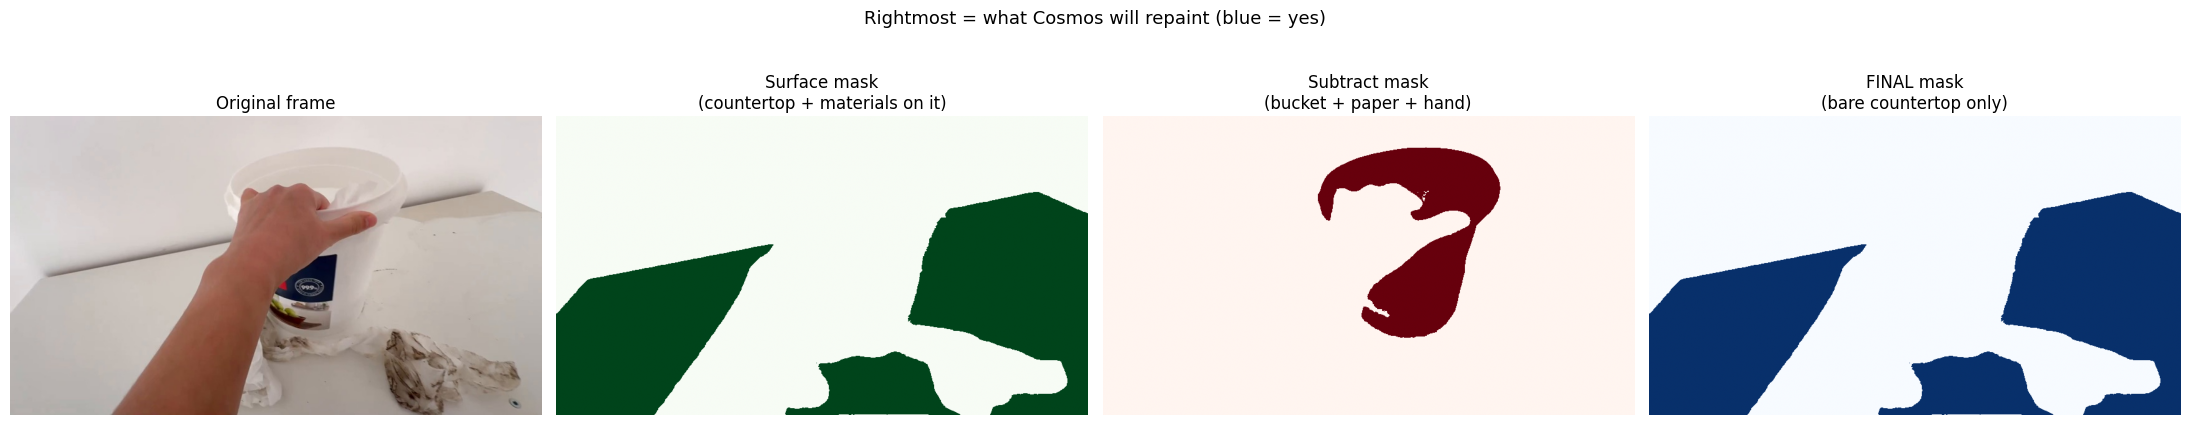
\includegraphics[width=\linewidth]{s11_mask_strip.png}\caption{building the subtraction mask}\end{subfigure}
\caption{Top: the four guidance maps for one frame. Edges keep the shapes, depth keeps the layout, color keeps the lighting, and the mask says where to paint. Bottom, left to right: original frame; SAM2 surface mask, which includes the materials on the counter; union of the bucket, paper and hand masks; final mask $M$ of Eq.~\ref{eq:mask}. Blue marks what the renderer is meant to repaint.}
\label{fig:maps}
\end{figure}

\begin{table}[t]
\centering
\caption{Control weights for Cosmos Transfer~2.5 as passed to the model (they sum to 0.9) and the failure that bounds each.}
\label{tab:weights}
\small
\begin{tabular}{@{}lrll@{}}
\toprule
Control & Weight & Too low & Too high \\
\midrule
edge  & 0.5   & objects lose shape & nothing changes \\
depth & 0.2   & layout drifts & scene flattens to a plane \\
vis (color) & 0.025 & none observed & recolor reverts \\
seg (mask)  & 0.175 & edits unlocalized & over-constrained \\
\bottomrule
\end{tabular}
\end{table}

\subsection{Generation}
\label{sec:generation}
Cosmos Transfer~2.5~\cite{cosmos25} renders $V'=G(V,p,\{c_j\},w)$ with 35 denoising steps and guidance scale 4; at 2 and 3 it often ignored the variation, and above 5 it followed the prompt but lost the room. Seeds were not fixed; outputs are 60 frames at $854\times480$ and 4~fps. Transfer preserves the source motion by construction, so action-level entries such as ``bucket tips over'' go to Cosmos Predict2 (2B, Video2World)~\cite{cosmospredict2}, which forecasts frames from a conditioning clip and a description of what happens next.
